\chapter{Estudio teórico de las bases del protocolo}\label{estudioteorico}

%
% PROBLEMA CUANTICO
%

\section{La computación cuántica y sus consecuencias en criptografía }

La criptografía es la base de nuestros sistemas informáticos ya que nos proporciona la seguridad necesaria para comunicarnos y tratar con cualquier tipo de información, de la más sensible a la menos. Las consecuencias de que no podamos confiar en esta seguridad sobre la que dependemos serían catastróficas, y justo eso es lo que amenaza hacer los ordenadores cuánticos.

Los ordenadores cuánticos no son sólo una amenaza por su velocidad y sus recursos propios sino que en 1994, Peter Shor publicó lo que hoy en día se conoce cómo algoritmo de Shor, posiblemente el más famoso de los algoritmos cuánticos a día de hoy. Este algoritmo permitiría resolver los problemas del logaritmo discreto y de la factorización de un número en tiempo polimonial. Estos problemas son la base de la mayoría de los protocolos criptográficos que utilizamos hoy en día por lo que una implementación en un ordenador cuántico de este algoritmo podría rebasar cualquier sistema de seguridad actual.

Uno de estos algoritmos en peligro es Diffie-Hellman, la base de la criptografía de clave pública. La seguridad de este protocolo reposa en la complejidad computacional del Problema Computacional Diffie-Hellman (CDHP por sus siglas en inglés) que trata lo que es conocido como el problema del logaritmo discreto (DLP).

\begin{problem}[Problema del logaritmo discreto]
    Dado $\alpha \in G$ y $\beta \in \langle \alpha \rangle$ encontrar el menor entero $x$ tal que $\alpha^x = \beta$. \cite{discrete-logarithm}
\end{problem}

Este problema ha sido adaptado de muchas formas, entre otras, a curvas elípticas. Esta adaptación toma la estructura de grupo de las curvas elípticas con la multiplicación escalar y aplica el concepto del logaritmo discreto, lo que se convierte en el ECDLP o Problema del Logaritmo Discreto en Curvas Elípticas.

Los algoritmos de Shor permitirían romper el problema del logaritmo discreto en tiempo polinomial en contraste con la complejidad exponencial de un algoritmo clásico,\footnote{Realmente, los algoritmos de Shor no son deterministas sino probabilísticos, es decir, no dan siempre el resultado correcto sino que lo encuentran un gran número de veces. No obstante, esto es suficiente para poner en peligro nuestra seguridad actual.} y aunque no se considera probable que se vayan a desarrollar ordenadores cuánticos que puedan implementar estos algoritmos en los próximos años (en la figura \ref{fig:expert-estimates} mostramos un gráfico proporcionado por el Global Risk Institute \cite{quantum-threat-timeline}), el proceso de migración utilizando los recursos que ahora mismo tenemos disponibles se estima que pueda tomar más de cinco años tomando de referencia transiciones previas \cite{coordinated-implementation-roadmap}.

\begin{figure}[!ht]
    \centering
    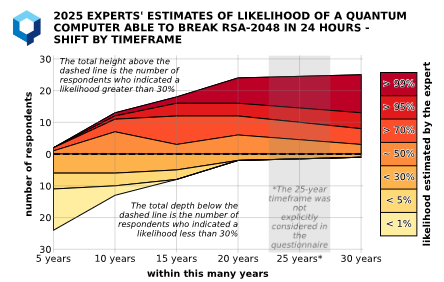
\includegraphics[width=0.75\linewidth]{img/expert-estimates.png}
    \caption{Un gráfico de área apilado que refleja los datos obtenidos, ofreciendo una visión clara de cómo las estimaciones cambian del corto al largo plazo: por cada rango horario, la altura total de la línea rayada indica el número de encuestados que estiman al menos una probabilidad del 30 por ciento.}
    \label{fig:expert-estimates}
\end{figure}

El National Institute of Standards and Technology o NIST, un organismo estadounidense perteneciente al ministerio de comercio que, entre otros objetivos, busca establecer unos estándares de seguridad capaces de hacer frente a la capacidad de los ordenadores cuánticos.

Esto es lo que se conoce como criptografía post-cuántica, no porque utilice algoritmos ni ordenadores cuánticos sino porque es resistenete a estos. Estos protocolos se basan en problemas matemáticos que deben ser resistentes tanto a ataques clásicos como a ataques cuánticos.

A lo largo de 2016 el NIST hizo una llamada general, presentó el concepto de criptografía post-cuántica y propuso unos plazos para encontrar candidatos a estandarización. La primera de las cuatro rondas se abrió en diciembre de ese año, cerrándose casi un año más tarde, en noviembre del 2017.

A finales de este año se presentaron los algoritmos que habían superado los requisitos mínimo de esta ronda, un total de 69. La segunda ronda se cerró en enero de 2019 y estuvo compuesta de 26 candidatos mientras que la tercera, en julio de 2020, se compuso de 15, 8 nominados y 7 alternos. La cuarta y última ronda se cerró en 2022, proponiendo los candidatos a estandarización \cite{nist-timeline}.


%
% SIDH vs SIKE
%

\section{SIDH vs SIKE}

SIKE (Super-singular Isogeny Key Encapsulation) \cite{sike-org}  \cite{SIKE} se postula como una adaptación de Diffie-Hellman con isogenias de curvas elípticas. Sin embargo, es posible que hayas oído hablar de otro protocolo que se llama, literalmente, Super-singular Isogeny Diffie-Hellman o SIDH. La duda que muchos se harán al encontrarse con estos dos conceptos es, razonablemente, cual es la diferencia entre uno y otro.

La respuesta es fácil, SIKE es una variación de SIDH. SIDH permite una mayor variabilidad al contar con un juego de parámetros libres, en concreto, el tamaño del primo. SIKE es, específicamente, la versión concreta presentada a las convocatorias del NIST. En ella, los autores definen cuatro posibles sets de parámetros: SIKEp434, SIKEp503, SIKEp610, SIKEp751 \cite{SIKE_specifications}.

\begin{table}[h]
    \centering
    \begin{tabular}{|p{0.17\linewidth}||p{0.17\linewidth}|p{0.16\linewidth}|p{0.16\linewidth}|p{0.16\linewidth}|}
         \hline
        Parámetros & Nivel de seguridad según el NIST & Clave privada (bytes) & Clave pública (bytes) & Secreto compartido (bytes)\\ \hline
        SIKEp434 & 1 & 374 & 330 & 16\\ \hline
        SIKEp503 & 2 & 424 & 378 & 24\\ \hline
        SIKEp610 & 3 & 524 & 462 & 24\\ \hline
        SIKEp751 & 5 & 644 & 564 & 32\\ \hline
    \end{tabular}
    \caption{Sets de parámetros proporcionados por SIKE}
    \label{tab:sike_parameters}
\end{table}

%
% FUNCIONAMIENTO DEL PROTOCOLO
%

\section{Funcionamiento del protocolo}

 \subsection{Resumen en lenguaje cercano}

 El protocolo presentado por de Feo, Jao y Plût utiliza el esquema clásico de Diffie-Hellman, la diferencia principal se encuentra en el contenido de la clave, en qué problema matemático se utiliza por detrás de estos esquemas ya probados para añadirle la seguridad que le falta a la criptografía clásica.
 
En vez del problema del logaritmo discreto como base de la seguridad y complejidad de SIKE, los autores han apostado por la composición de funciones, en concreto, de isogenias supersingulares.

Para conseguir el secreto conjunto, los usuarios parten de una curva pública común. Cada uno por separado, le aplican a esta misma curva una serie de transformaciones llegando a unas curvas intermedias independientes. Llegados este punto, intercambian las imágenes de estos puntos públicos originales que utilizarán para continuar las transformaciones. De esta forma consiguen llegar a un secreto común sin haber compartido las isogenias que han utilizado.

En un primer momento, se consideró que estos puntos intermedios que se comparten en claro no suponían un peligro para el secreto, por ello el protocolo pasó hasta la tercera ronda del NIST. Sin embargo, en Julio de 2022, Wouter Castryck y Thomas Decru publicaron un ataque efectivo contra el protocolo utilizando estos puntos \cite{efficient_attack}.

\begin{comment}
%
% PRUEBA DE IDENTIDAD
%

\subsection{Prueba de identidad}

El protocolo de identidad ideado por De Feo, Jao y Plût se basa en el siguiente esquema:

\begin{figure}[!ht]
    \centering
    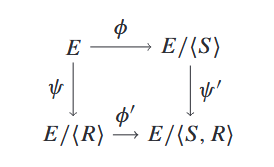
\includegraphics[width=0.3\linewidth]{img/Zero-knowledge graph.png}
    \caption{Diagrama sobre el que reposa la idea de la prueba de identidad}
    \label{fig:proof_of_identity}
\end{figure}

donde $\langle S \rangle$ es el kernel de la isogenia secreta $\phi$ de grado $l_A^{e_A}$ y $\langle R \rangle$ es un grupo cíclico de orden $l_B^{e_B}$. Los usuarios, utilizaremos Alice y Bob, pueden computarlo fácilmente utilizando las fórmulas de Vélu y calculando las isogenias a partir de las imágenes de los puntos.

El problema es entonces qué puede Alice desvelar del diagrama para demonstrar su identidad sin comprometer su secreto $\phi$. No puede ser $(\psi, \phi’)$ ó $(\psi’, \phi’)$ ya que estos permiten fácilmente computar $Ker(\phi)$. Finalmente, nos decantamos por $(\psi, \psi’)$.

\subsubsection{Parámetros públicos y secretos}

\begin{description}
    \item Parámetros públicos
        \begin{enumerate}
            \item Curvas elípticas supersingulares $E, E/\langle S \rangle$.
            \item Generadores $P,Q$ de $E[l_B^{e_B}]$ y sus imágenes $\phi(P),\phi(Q)$.
        \end{enumerate}
    \item Parámetros secretos
        \begin{enumerate}
            \item Punto de $l_A^{e_A}$-torsión $S$ que define
            \item La isogenia $\phi : E \to E/\langle S \rangle$.
        \end{enumerate}
\end{description}

\subsubsection{Pasos del protocolo}

Los siguientes pasos se repetirán un número $m$ de veces.

\begin{enumerate}
    \item Alice escoge un punto aleatorio $l_B^{e_B}$-torsión $R$ y computa el diagrama anterior.
    \item Alice le envía a Bob las curvas $E / \langle R \rangle, E/ \langle S,R \rangle$.
    \item Bob escoge un bit aleatorio $b$ y se lo envía a Alice.
        \begin{itemize}
            \item Si $b = 0$, Alice revela $R, \phi(R')$ y, si tienen orden $l_B^{e_B}$, Bob genera los kernel de las isogenias $E \to E / \langle R \rangle, E/\langle S \rangle \to E/ \langle S,R \rangle$, respectivamente.
            \item Si $b=1$, Alice revela $\psi(S)$ y, si tiene orden $l_A^{e_A}$, Bob genera el kernel de la isogenia $E / \langle R \rangle \to E/ \langle S,R \rangle$.
        \end{itemize}
\end{enumerate}
\end{comment}

%
% INTERCAMBIO DE CLAVES
%

\subsection{Intercambio de claves}

El intercambio de claves que propone SIKE es una adaptación de Diffie-Hellman en el que los usuarios computan isogenias individuales y a partir de estas crean la clave compartida.

\subsubsection{Parámetros}

Empezamos definiendo los siguientes parámetros públicos compartidos:

\begin{enumerate}
    \item Un primo $p=l_A^{e_A} \cdot l_B^{e_B} \cdot f \pm 1$.
    \item Una curva elíptica $E_0$ definida sobre $\mathbb{F}_{p^2}$.
    \item Un par de puntos $\{ P_A,Q_A \}, \{ P_B,Q_B \}$ para Alice y Bob respectivamente donde $\langle P_A,Q_A \rangle = E[l_A^{e_A}]$ , análogamente con $\langle P_B, Q_B \rangle$.
\end{enumerate}

\subsubsection{Pasos del protocolo}

Una vez establecemos estos valores, comienza el proceso de intercambio de clave. Trataremos sólo los pasos de Alice por simplificar la explicación, ya que Bob sigue el mismo proceso, aunque los valores específicos cambien.

Alice escoge un par de valores cualesquiera $m_A,n_A$ pertenecientes al grupo $\mathbb{Z}/ l_A^{e_A} \mathbb{Z}$, con ambos no divisibles por $l_A$. A partir de estos dos valores computa una primera isogenia $\phi_A$ con

\[Ker(\phi_A) = K_A := \langle [m_A]P_A + [n_A]Q_A \rangle\]

Una vez tiene definida este morfismo, computa las imágenes de los puntos base de Bob, es decir, $\phi_A(P_B), \phi_A(Q_B)$. En este punto del proceso, Alice y Bob intercambian la siguiente tupla de información $(E_A, \{ \phi_A(P_B), \phi_A(Q_B) \})$ y recibe una equivalente de parte de Bob. A partir de estos puntos intermedios, Alice calculará una nueva isogenia $\phi_A’$ con

 \[Ker(\phi_A) = K_A := \langle [m_A]\phi_B(P_A) + [n_A]\phi_b(Q_A) \rangle\]
 
De esta forma consiguen llegar a un $j$-invariante común que usarán de clave compartida.

 \[E_{AB} = \phi_B’(\phi_A(E_0)) = \phi_A’(\phi_B(E_0)) \rangle\]

Para simplificar la comprensión del protocolo, incluimos el esquema en la figura \ref{fig:diagrama}.

\newpage
\begin{figure}[!h]
    \centering
    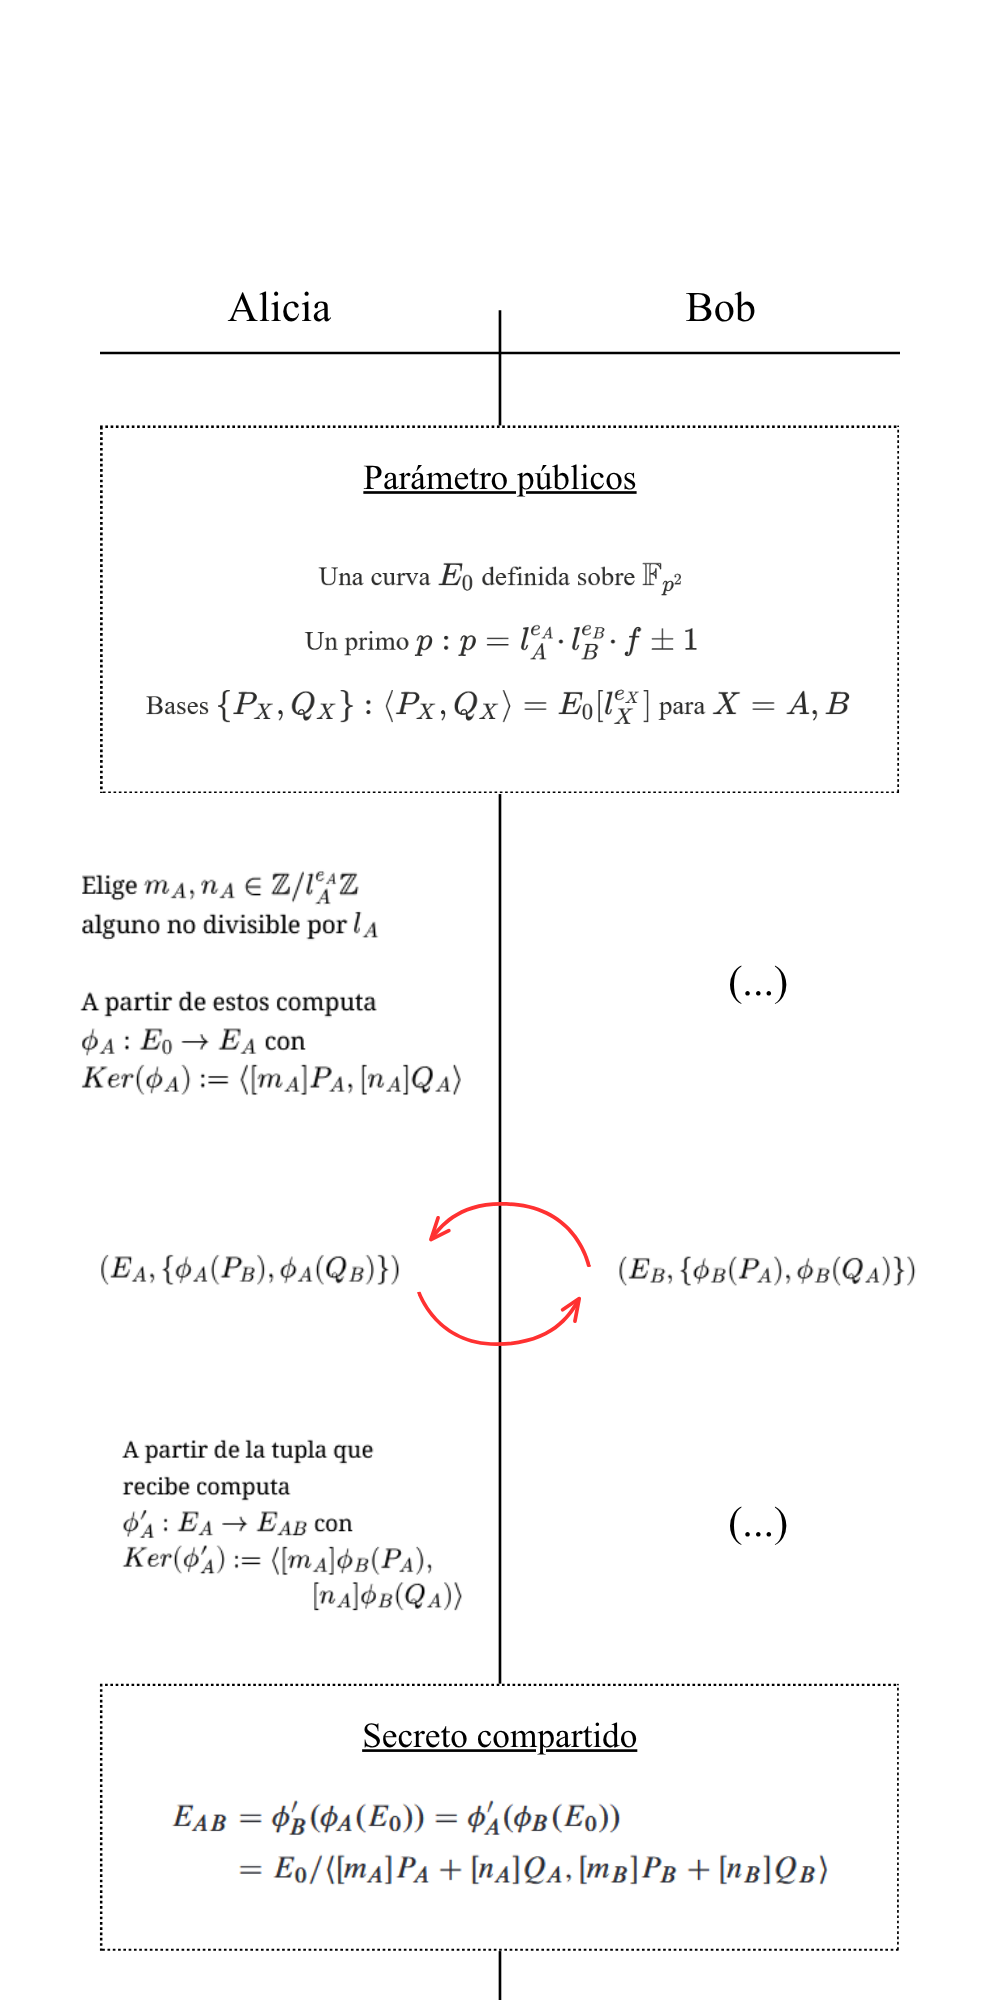
\includegraphics[width=0.75\linewidth]{img/Key exchange.png}
    \caption{Diagrama explicativo del protocolo de intercambio de clave}
    \label{fig:diagrama}
\end{figure}

\newpage
\subsubsection{Visualización del protocolo}

Comprender cómo funciona el intercambio de claves resulta mucho más sencillo si vemos el viaje que Alice y Bob realizan a través de un grafo de isogenias concreto. Pongamos de ejemplo el primo $p = 433$. En la figura \ref{fig:grafos-base} encontramos los grafos 2 y 3 isogenias de este primo por los datos proporcionados por la base de datos \textit{Isogeny graphs of supersingular elliptic curves} \cite{isogeny-graphs-ddbb}.

\begin{figure}[!h]
\begin{subfigure}[h]{0.4\linewidth}
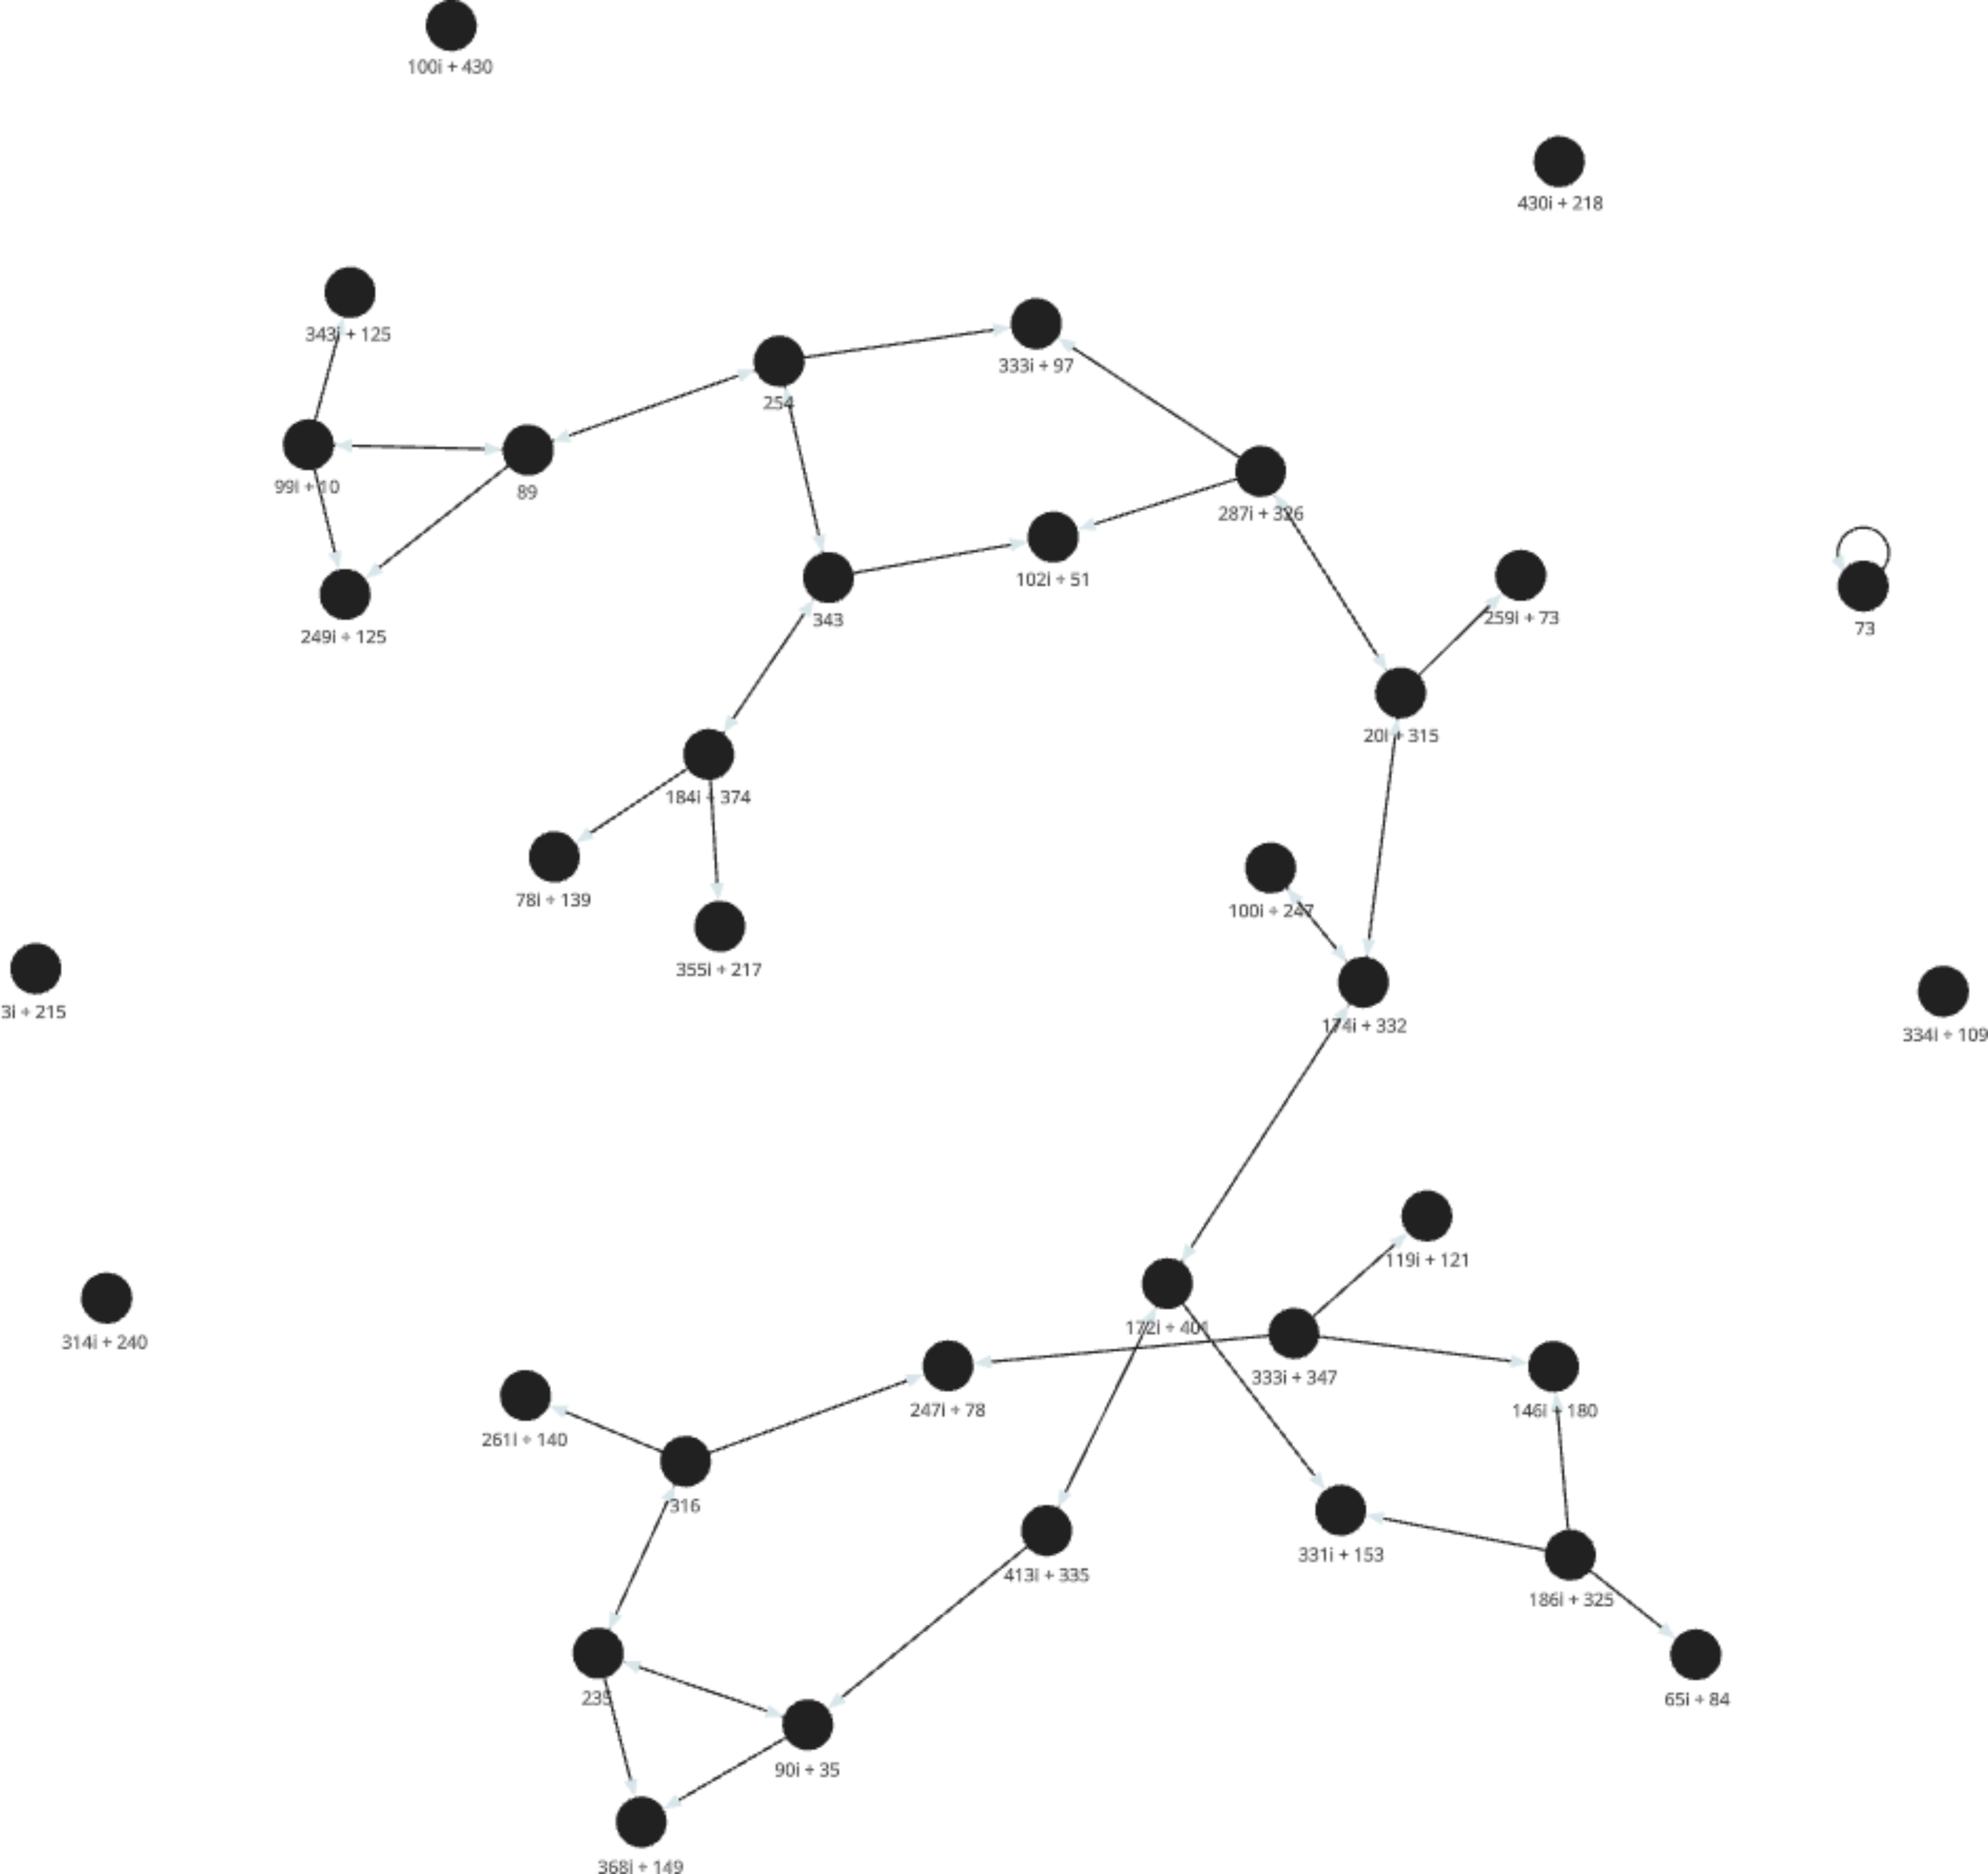
\includegraphics[width=\linewidth]{img/2-isogeny/2-isogeny.png}
\caption{Grafo de 2-isogenias}
\end{subfigure}
\hfill
\begin{subfigure}[h]{0.4\linewidth}
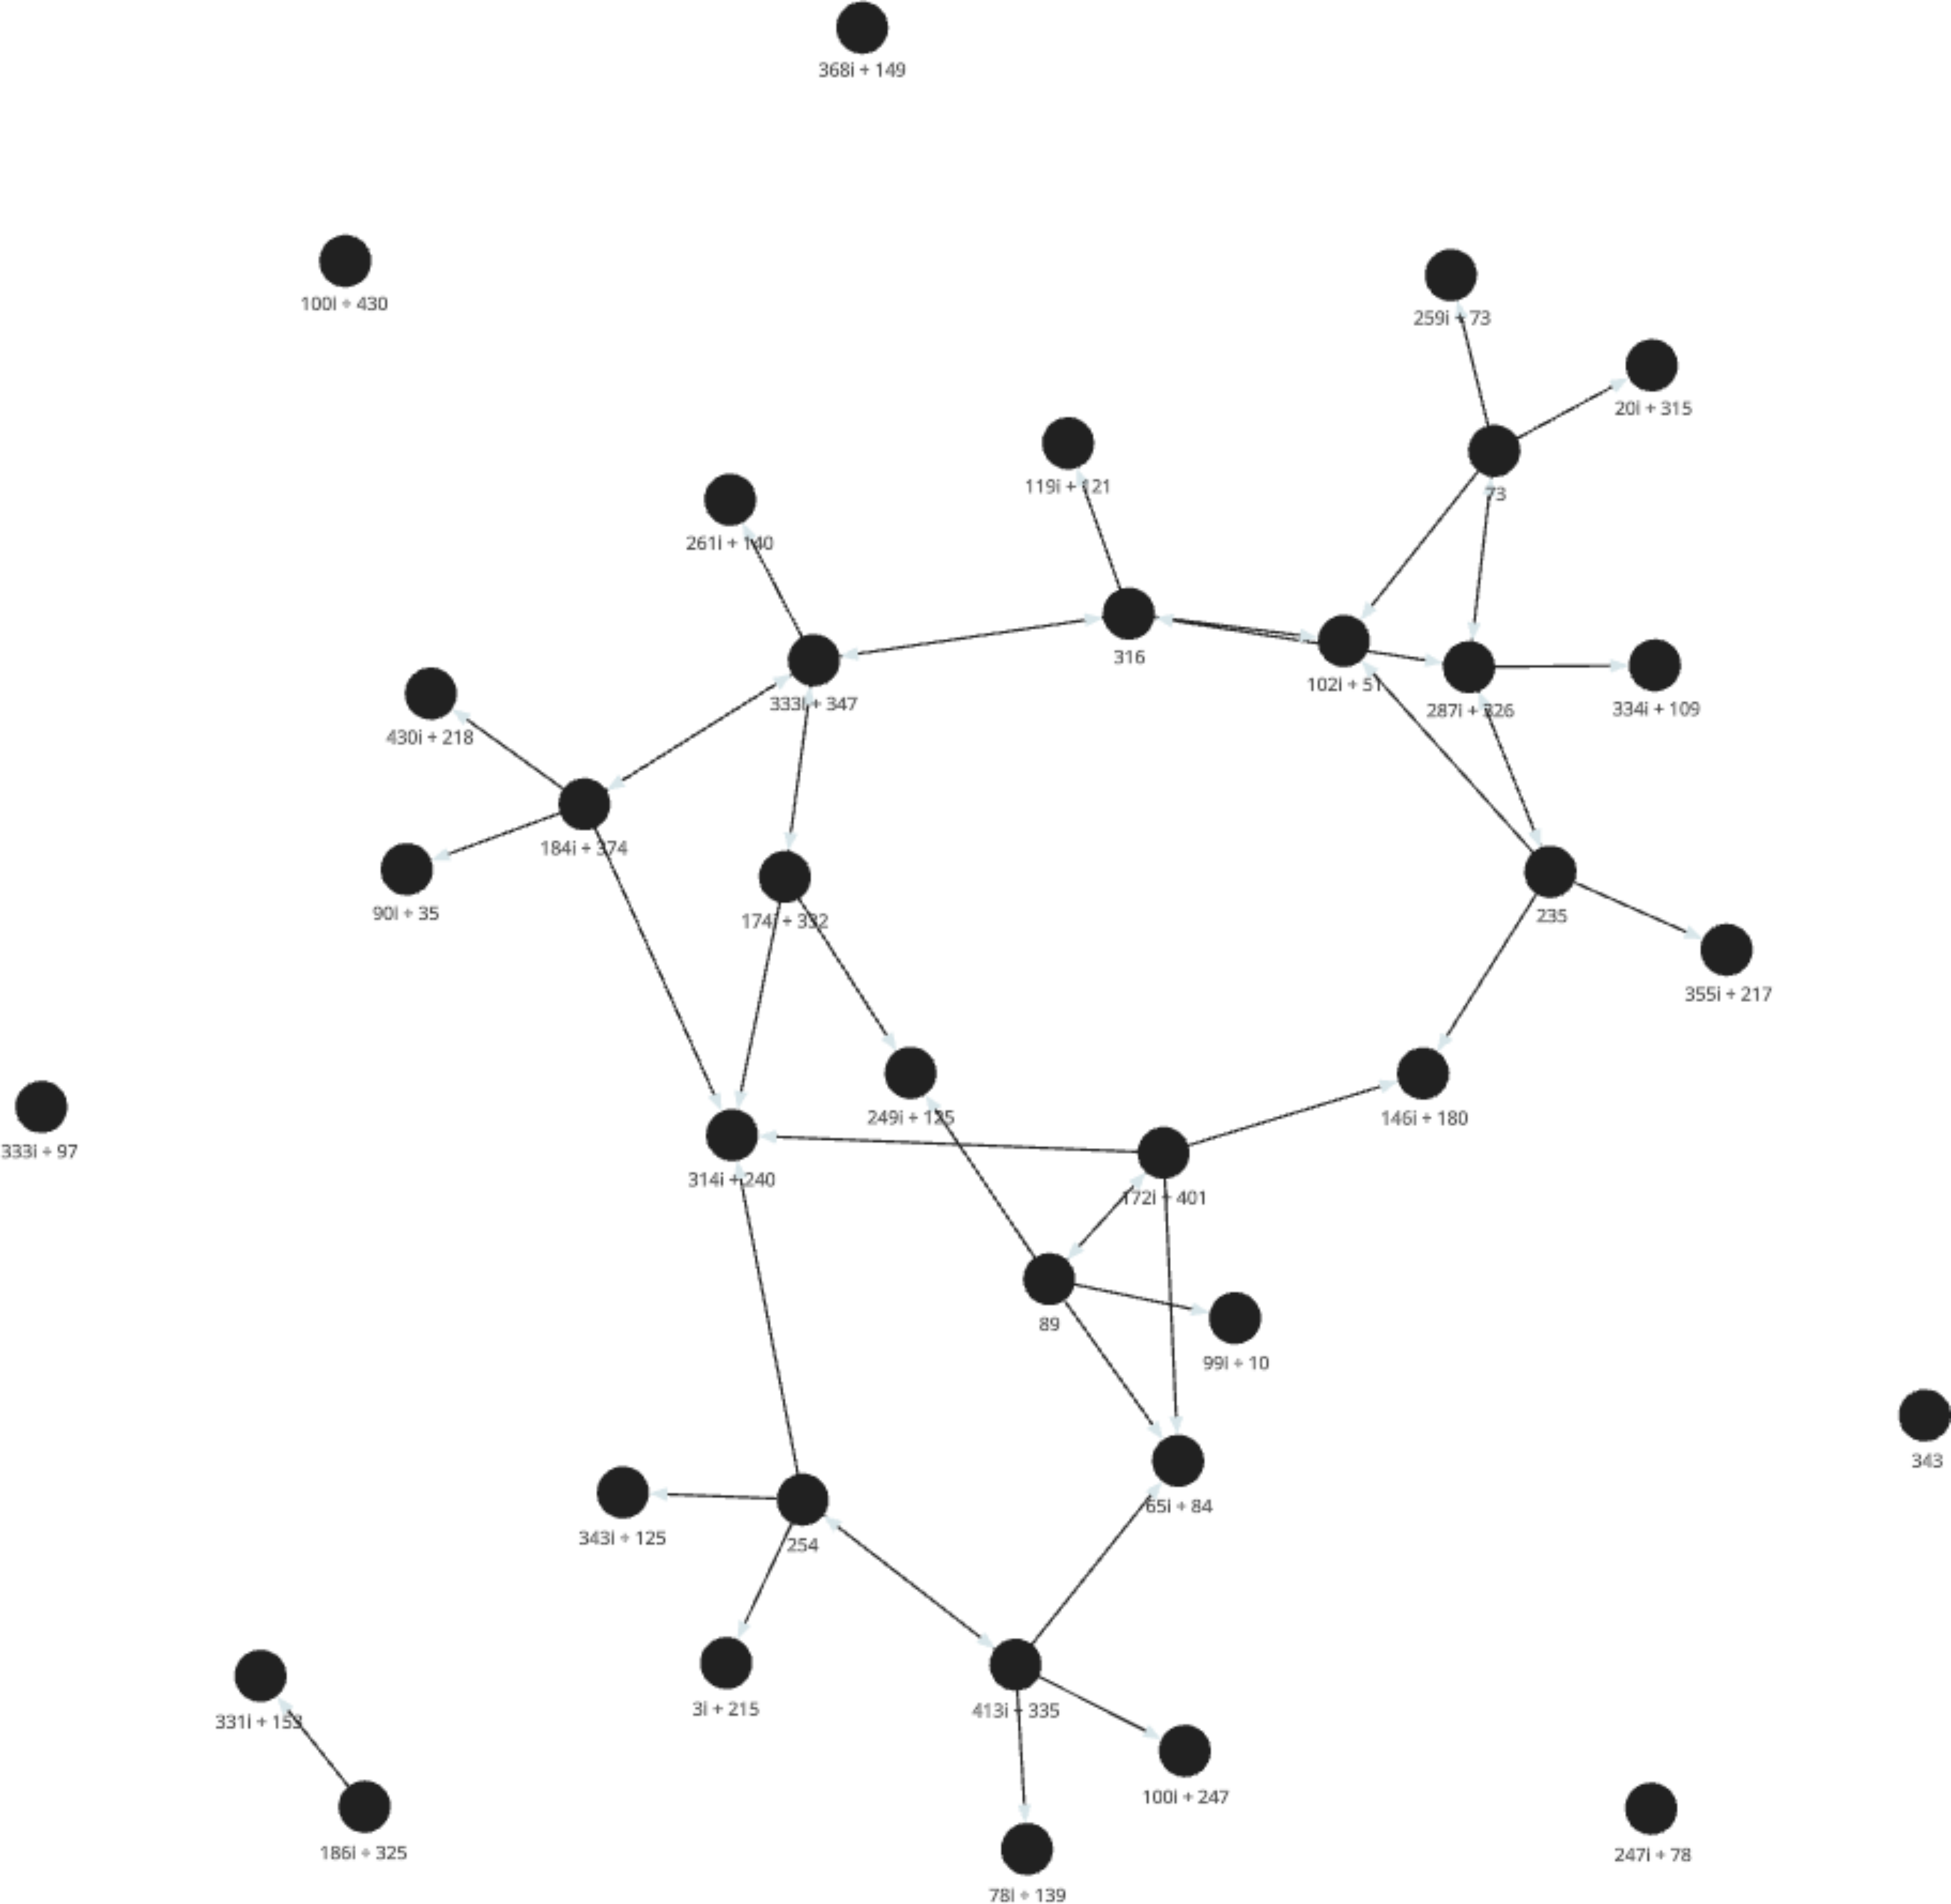
\includegraphics[width=\linewidth]{img/3-isogeny/3-isogeny.png}
\caption{Grafo de 3-isogenias}
\end{subfigure}
\caption{Grafos de isogenias para $p=433$}
\label{fig:grafos-base}
\end{figure}

Al calcular las isogenias intermedias propias de Alice y Bob, estos se desplazan por el grafo de isogenias. La factorización del primo escogido tiene gran importancia en este punto, ya que va a definir cómo estos se mueven por el grafo. Hemos escogido el primo $433$ que se puede factorizar de la siguiente forma $p = 433 = 2^4 \cdot 3^3 + 1$. Tenemos entonces que $l_A = 2, e_A = 4$ y $l_B = 3, e_B = 3$\footnote{Puede ser al revés, pero en este ejemplo trataremos con estos valores.}. Alice entonces, se desplazará a través de 4 nodos en el grafo de 2-isogenias mientras que Bob atravesará 3 nodos en el de 3-isogenias. En la figura \ref{fig:grafos-intermedio} encontramos un ejemplo de esta primera parte del camino.

\begin{figure}[!h]
\begin{subfigure}[h]{0.4\linewidth}
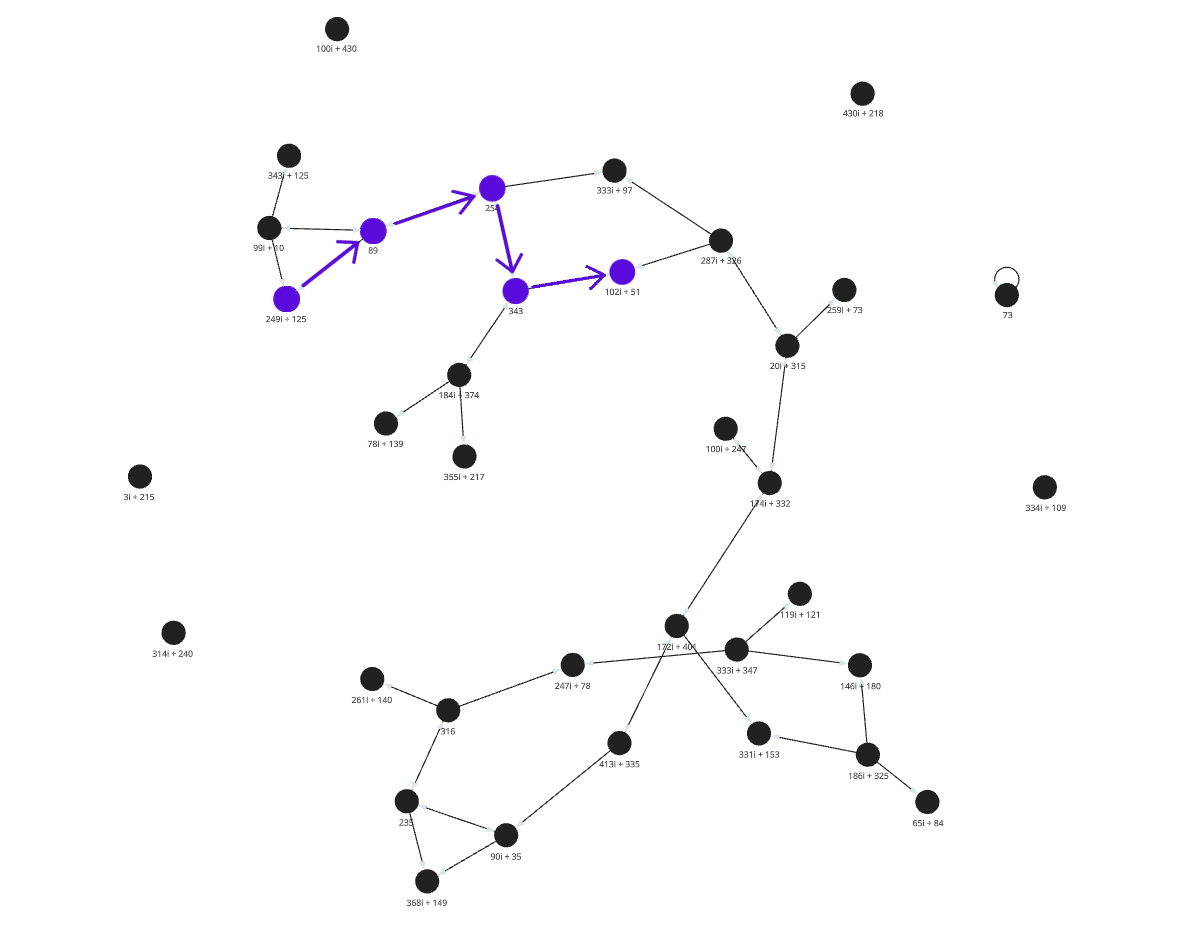
\includegraphics[width=\linewidth]{img/2-isogeny/step4.png}
\caption{Camino por el grafo de 2-isogenias}
\end{subfigure}
\hfill
\begin{subfigure}[h]{0.4\linewidth}
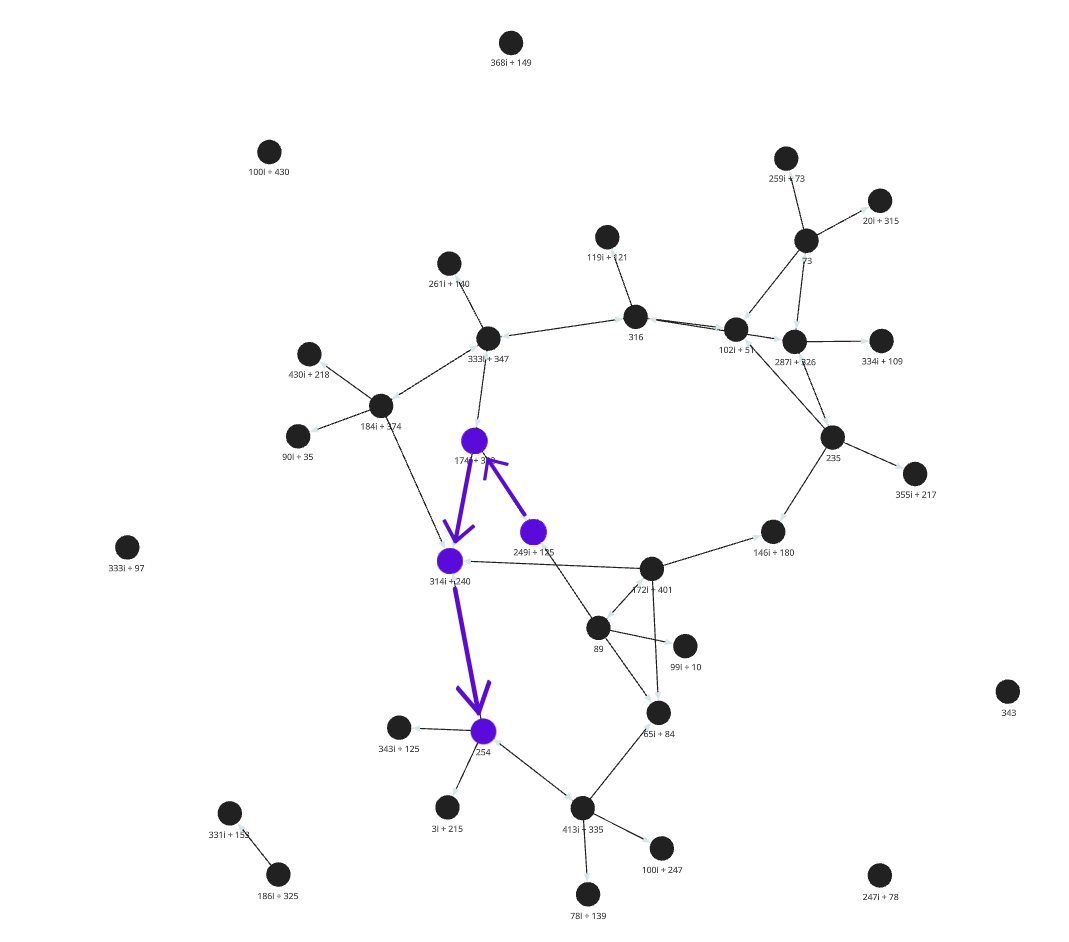
\includegraphics[width=\linewidth]{img/3-isogeny/step3.png}
\caption{Camino por el grafo de 3-isogenias}
\end{subfigure}
\caption{Caminos por los grafos de isogenias para $p=433$}
\label{fig:grafos-intermedio}
\end{figure}

Es en este punto en el que Alice y Bob calculan las imágenes de los puntos iniciales del otro y se las intercambian. Una vez tienen estos puntos intermedios, vuelven a desplazarse a través del grafo para llegar a una misma curva $E_{AB}$. En la figura \ref{fig:grafos-final} mostramos esta segunda parte del viaje mientras que en la \ref{fig:grafos-invariante} mostramos en concreto el nodo final del desplazamiento.

\begin{figure}[!h]
\begin{subfigure}[h]{0.4\linewidth}
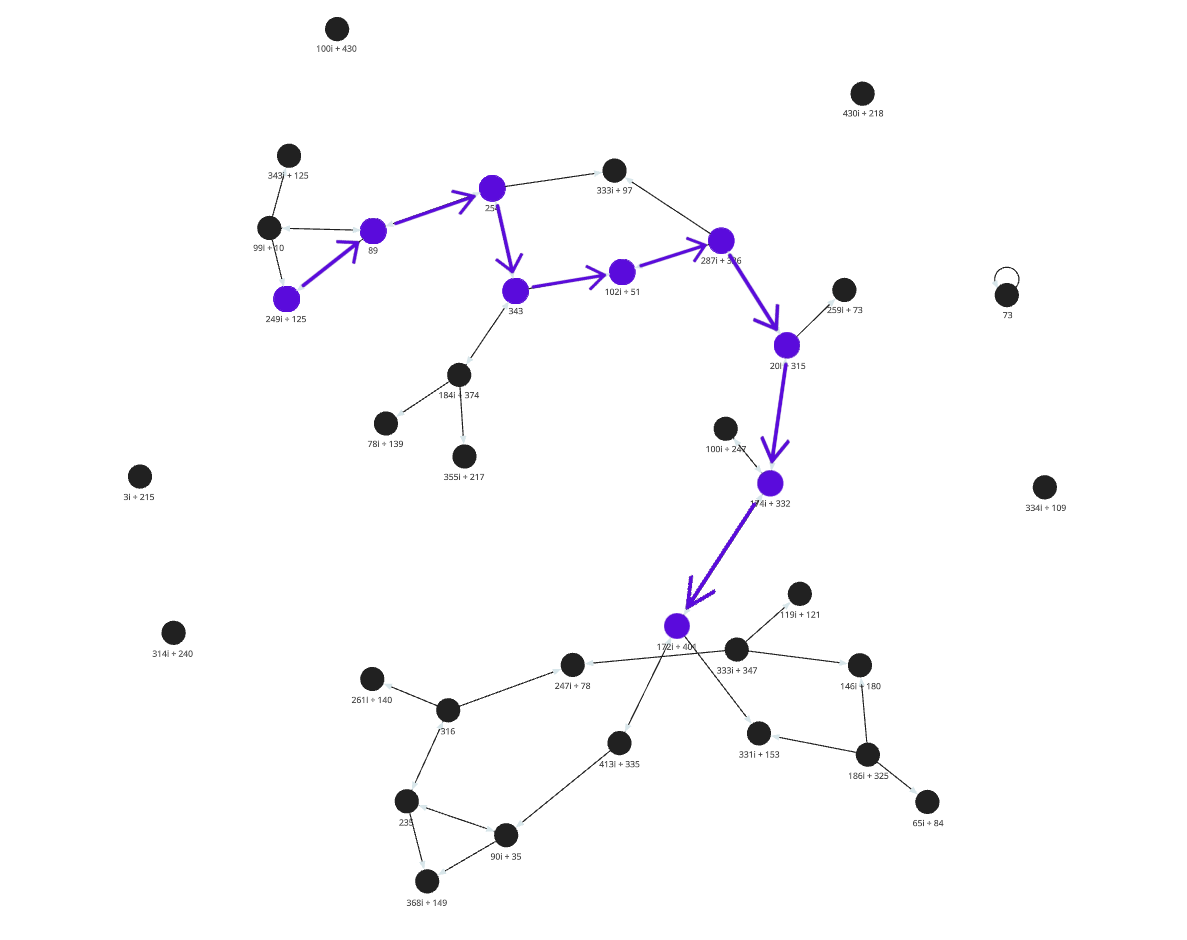
\includegraphics[width=\linewidth]{img/2-isogeny/step8.png}
\caption{Camino final por el grafo de 2-isogenias}
\end{subfigure}
\hfill
\begin{subfigure}[h]{0.4\linewidth}
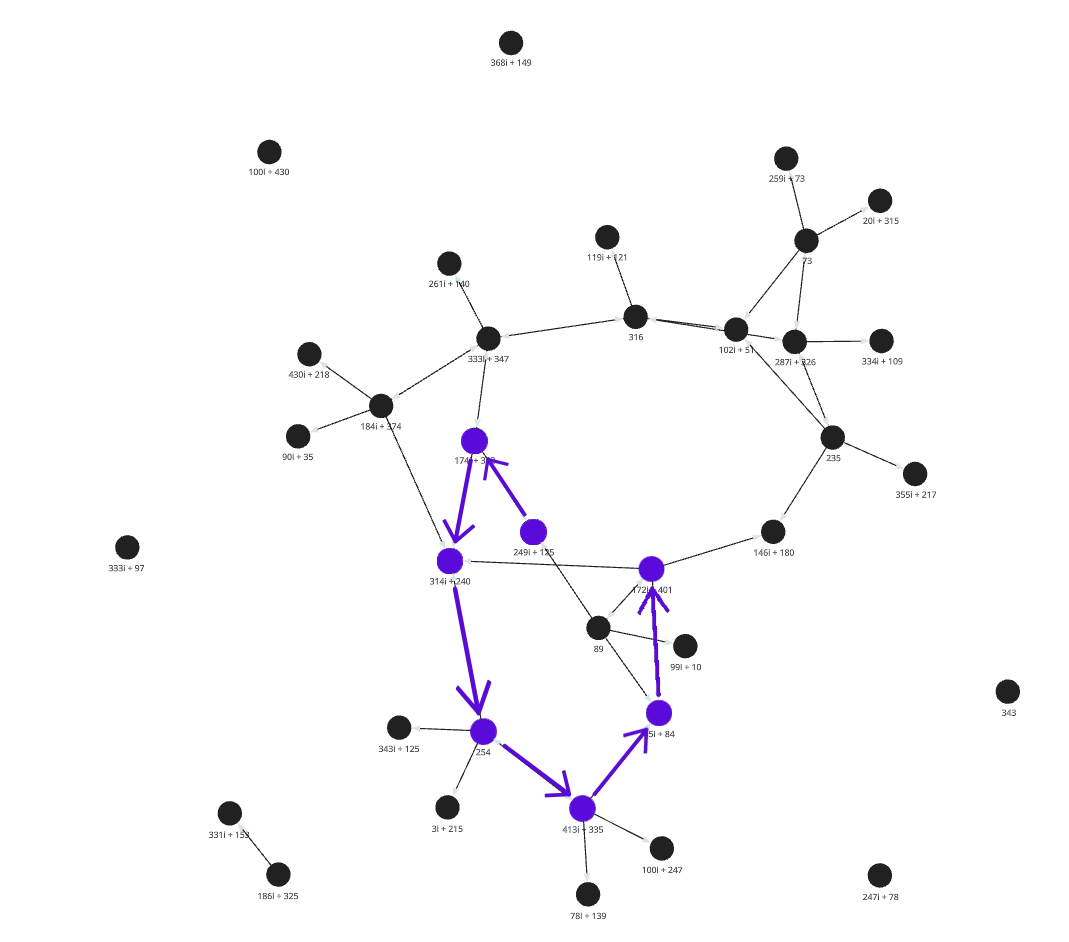
\includegraphics[width=\linewidth]{img/3-isogeny/step6.png}
\caption{Camino final por el grafo de 3-isogenias}
\end{subfigure}
\caption{Caminos finales por los grafos de isogenias para $p=433$}
\label{fig:grafos-final}
\end{figure}

\begin{figure}[!h]
\begin{subfigure}[h]{0.4\linewidth}
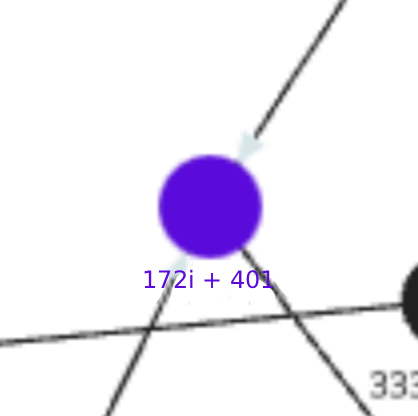
\includegraphics[width=\linewidth]{img/2-isogeny/closeup.png}
\caption{$j$-invariante final en el grafo 2-isogenias}
\end{subfigure}
\hfill
\begin{subfigure}[h]{0.4\linewidth}

\includegraphics[width=\linewidth]{img/3-isogeny/closeup.png}
\caption{$j$-invariante final en el grafo 3-isogenias}
\end{subfigure}
\caption{$j$-invariante final en los grafos.}
\label{fig:grafos-invariante}
\end{figure}


\subsubsection{Implementación}

A la hora de simular este intercambio de clave para llegar al secreto compartido, hemos seguido los pasos proporcionados por los desarrolladores de la implementación Java \cite{sike-java}. A continuación, proporcionaremos el código exacto para los pasos que hemos explicado anteriormente.

El proceso de encapsulación comienza con Bob generando una clave. Tenemos a elegir entre los cuatro conjuntos de parámetros predefinidos y una implementación optimizada o una de referencia. Vamos a utilizar la implementación optimizada dado que no vamos a tratar con el código fuente sino que vamos a utilizarlo, nos interesa más la rapidez que la legibilidad del código.

\begin{verbatim}
SikeParam sikeParam = new SikeParamP434(ImplementationType.OPTIMIZED);
KeyGenerator keyGenerator = new KeyGenerator(sikeParam);
KeyPair keyPairB = keyGenerator.generateKeyPair(Party.BOB);
\end{verbatim}

A continuación comienza el proceso de intercambio de claves propiamente dicho. Alice genera su paso intermedio, la entidad \verb|sike|, y, con la clave pública de Bob, la encapsula.

\begin{verbatim}
Sike sike = new Sike(sikeParam);
EncapsulationResult encapsulationResult 
    = sike.encapsulate(keyPairB.getPublic());
\end{verbatim}

Alice calcula el secreto compartido, la curva final, y el mensaje cifrado.

\begin{verbatim}
byte[] secretA = encapsulationResult.getSecret();
EncryptedMessage encryptedMessage 
    = encapsulationResult.getEncryptedMessage();
\end{verbatim}

Bob recibe el mensaje cifrado \verb|encryptedMessage| como un array de bytes y utiliza la clave pública para el descifrado, obteniendo así su clave secreta. 

\begin{verbatim}
byte[] encodedMessage = encryptedMessage.getEncoded();
EncryptedMessage transportedMessage 
    = new EncryptedMessage(sikeParam, encodedMessage);
byte[] secretB = sike.decapsulate(
                    keyPairB.getPrivate(), 
                    keyPairB.getPublic(), 
                    transportedMessage
                );
\end{verbatim}

Ahora tenemos dos secretos, los correspondientes a Alice y Bob, \verb|secretA| y \verb|secretB| respectivamente. La implementación proporcionada por Wultra funciona de manera correcta y estos dos secretos efectivamente coinciden. Sin embargo, en nuestro proyecto, para añadir una capa de seguridad extra, comprobamos que estos dos coincidan antes de continuar con el cifrado del mensaje.

%
% CIFRADO
%

\subsection{Cifrado}

Una vez tenemos el secreto compartido, veamos cómo funciona el cifrado con SIKE.

\begin{enumerate}
    \item \textbf{Preparación}: se establecen los parámetros públicos, esto es, los parámetros comentados en el apartado anterior, además de la familia de funciones resumen $\mathcal{H} = \{ H_k : k \in K \}$, donde $K$ es un conjunto finito y cada $H_k$ es una función resumen distinta. SIKE no utiliza una función resumen reconocida como SHA-3, sino que incluye un elemento de variabilidad en el cifrado al tener esta familia de funciones y para cada cifrado elegir una diferente de manera pseudo-aleatoria.
    
    \item \textbf{Generación de la clave}: seguimos el protocolo de intercambio de clave de donde obtenemos
    \begin{itemize}
        \item La clave pública $(E_A, \{ P_A, Q_A \})$
        \item Un elemento secreto pseudo-aleatorio $k$
        \item La curva $E_{AB}$ compartida.
    \end{itemize}

    \item \textbf{Cifrado}: el cifrado de SIKE consiste en una multiplicación lógica. Para ello, antes de nada, calculamos el $j$-invariante de la curva compartida $E_{AB}$
        \[ j = j(E_{AB}) \]
    del que calculamos el resumen utilizando una función resumen perteneciente a la familia $\mathcal H$ escogida pseudo-aleatoriamente. Es por esto por lo que un elemento $k \in K$ forma parte de la clave privada. 
        \[ h = H_k(j) \]
    una vez ya tenemos calculado el resumen del $j$-invariante, hacemos la multiplicación lógica con el mensaje en claro $m$ para obtener el mensaje cifrado $c$
        \[ c = h \oplus m \]

    \item \textbf{Descifrado}: como tanto el elemento $k$ como la curva $E_{AB}$ forman parte del secreto compartido, para conseguir el texto en claro a partir del texto cifrado tan solo tenemos que deshacer los pasos del cifrado. Calculamos $j$ y $h$ igual que antes
        \[ j = j(E_{AB}), \, h = H_k(j) \]
    y luego simplemente calculamos la multiplicación lógica del mensaje cifrado $c$ para encontrar $m$
        \[ m = h \oplus c \]
\end{enumerate}

Como podemos ver, el cifrado es simplemente una multiplicación lógica, la seguridad del cifrado reposa íntegramente sobre la dificultad de computar el secreto compartido.

\subsubsection{Implementación}

A la hora de implementar el cifrado, hemos simplificado la elección de la función hash. En vez de generarla pseudo-aleatoriamente con un parámetro $k$ perteneciente a la clave pública, utilizamos siempre la misma, una instancia de \verb|SHAKE256|, derivada de SHA-3. A continuación, analizamos el funcionamiento del método implementado.

En primer lugar, a partir del mensaje original o $m$, generamos el array de bytes que lo representa.

\begin{verbatim}
public byte[] encode(SikeEntity sikeEntity) {
    String message = sikeEntity.getOriginalMessage();
    byte[] messageBytes = message.getBytes(StandardCharsets.UTF_8);
\end{verbatim}

A continuación, creamos una instancia \verb|SHAKE| y la actualizamos con el secreto compartido, es decir, hacemos el hash del secreto compartido.

\begin{verbatim}
    SHAKEDigest shake = new SHAKEDigest(256);
    byte[] keyBytes = sikeEntity.getKeyBytes();
    shake.update(keyBytes, 0, keyBytes.length);
\end{verbatim}

Una vez tenemos los dos arrays de bytes, generamos el mensaje cifrado o $c$ haciendo la multiplicación lógica de estos dos.

\begin{verbatim}
    byte[] encodedMessage = new byte[messageBytes.length];
    for (int i = 0; i < messageBytes.length; i++) {
        encodedMessage[i] = (byte) (keyBytes[i%16] ^ messageBytes[i]);
    }
\end{verbatim}

Este producto final, es el mensaje cifrado que devolvemos.

\begin{verbatim}
    return encodedMessage;
}
\end{verbatim}

El método que calcula el mensaje en claro es idéntico al anterior, la única diferencia es que en vez del mensaje original utilizamos el mensaje cifrado que acabamos de calcular y en vez de devolver el array de bytes del mensaje cifrado, devolvemos un \verb|String| con el mensaje en claro final.

\begin{verbatim}
public String decode(SikeEntity sikeEntity) {
    byte[] encodedMessage = sikeEntity.getEncodedMessage();

    SHAKEDigest shake = new SHAKEDigest(256);
    byte[] keyBytes = sikeEntity.getKeyBytes();
    shake.update(keyBytes, 0, keyBytes.length);

    byte[] decodedMessageBytes = new byte[encodedMessage.length];
    for (int i = 0; i < encodedMessage.length; i++) {
        decodedMessageBytes[i] = (byte) (keyBytes[i%16] 
                                    ^ encodedMessage[i]);
    }

    return new String(decodedMessageBytes);
}
\end{verbatim}

Al igual que en la fase de intercambio de llaves no es realmente necesario comprobar que el secreto compartido se haya calculado correctamente pero igualmente lo hacemos. A la hora de cifrar y descifrar el mensaje también incluimos una comprobación de que todo ha ido correcto.

%
% SEGURIDAD
%

\section{Seguridad}

Al contrario que la criptografía de curvas elípticas clásica, SIDH no se basa en el problema del logaritmo discreto, sino en un problema de complejidad clásico llamado "claw finding problem" (poblema de la pinza, de aquí en adelante) que, en vez de buscar una factorización, busca dos funciones con un mismo valor en dos puntos cualesquiera.

\begin{definition}[Oráculo cuántico estándar]
    En un entorno cuántico, un oráculo de dos funciones $f,g$ se define como
    \[ O_{f,g}: |p,z,w\rangle \to |p,z\oplus P(p)\,\,(\,\text{mod} |Z|\,),w\rangle \]
    donde $p\in W\cup Y, z\in Z,w$ es el espacio de trabajo, y
    \[ P(p) = \begin{cases}
       f(p) &\text{si } p \in X \\
       g(p) &\text{si } p \in Y
    \end{cases} \]
\end{definition}

\begin{problem}[Problema de la pinza]
    Dadas dos funciones $f:X:=[N] \to Z$ y $g:Y:=[M] \to Z$ mediante un oráculo con $N \geq M$ y $Z=[\,|Z|\,],$ encontrar un par $(x,y) \in X \times Y$ para los cuales $f(x) = g(Y)$, si existe. \cite{claw-finding-algorithms}
\end{problem}

Este problema, en vez de tratar con la propia curva trata con la interacción entre curvas.

\begin{table}[!ht]
    \centering
    \begin{tabular}{ |p{0.25\linewidth}||p{0.33\linewidth}|p{0.33\linewidth}|}
        \hline
        & ECDH & SIDH \\
        \hline
        Elementos & Puntos de la curva & $j$-invariante \\
        Computación & $k,P \to [k]P$ & $\phi,E \to \phi(E)$ \\
        Secreto & Escalar $k$ & Isogenia $\phi$ \\
        Problema & Logaritmo discreto & Problema de la pinza \\
        \hline
    \end{tabular}
    \caption{Comparación con la criptografía clásica de curvas elípticas}
    \label{tab:ecdh-vs-sidh}
    \cite{sidh-sike}
\end{table}

Cuando primero se ideó SIKE, el mejor ataque contra el protocolo era atacar directamente el problema de la pinza, lo que conlleva complejidad $O(p^{1/4})$ en un contexto clásico y $O(p^{1/6})$ en uno cuántico. Esto permitía tener una gran seguridad con una clave pública bastante pequeña. SIKEp751, la propuesta de mayor tamaño de SIKE, tiene una clave pública de 564 bytes mientras que McEliece, otro protocolo propuesto, tiene el mismo nivel de seguridad, el máximo que otorga el NIST, pero con una clave pública de 1044992 bytes. 

%
% DESCALIFICACIÓN DEL NIST
%

\section{Descalificación del NIST}\label{sec:estudioteorico:descalificacion}

Como ya hemos mencionado en varias ocasiones, SIKE ha sido descalificado del NIST al haberse encontrado un ataque clásico no genérico que explota los puntos auxiliares para encontrar un camino alternativo a la curva compartida secreta.

Este ataque publicado no fue el primer acercamiento al diseño de un ataque no genérico contra SIDH. En 2017, Petit publicó un algoritmo que permitía encontrar el secreto para algunos casos particulares de SIDH \cite{petit}, sin embargo, el protocolo de forma general y SIKE en particular todavía se consideraban seguros.

El ataque publicado el 22 de julio de 2022 por Castryck y Decru \cite{efficient_attack} permitía, en ese momento, romper SIKEp434 en una hora y SIKEp751, el primo más grande contemplado por SIKE con el nivel más alto de seguridad, en unas 20 usando un ordenador de núcleo único. 

Dado al atractivo de SIKE por su pequeño tamaño de clave y de texto cifrado se intentó en un primer momento salvar a SIDH aumentando el tamaño de los parámetros.  Entre otras propuestas encontramos \textit{Masked-degree SIDH} \cite{masked-degree-sidh} y \textit{SIDH with masked torsion point images} \cite{masked-torsion-sidh}. Lamentablemente, con mejoras posteriores los tiempos del ataque eficiente se reducen a menos de un minuto y menos de una hora, por lo que SIKE fue finalmente descalificado.

La caída en desgracia de SIKE no termina ahí, ya que sigue existiendo SIDH que, como hemos visto, es la generalización de la propuesta al NIST. No obstante, ese mismo año en agosto, Maino y Martindale publican \textit{An attack on SIDH with arbitrary starting curve} que generaliza el ataque de Castryck y Decru a cualquier esquema de SIDH que publique los puntos auxiliares.